%!TEX root = dissertation.tex
\chapter{Applications}
\label{chap:apps}
In this chapter, we present the experimental results in Publications~\cp{paperDRIFT}, \cp{paperKFSECG}, \cp{paperKFSECGCONF}, \cp{paperSSDGP}, and~\cp{paperMARITIME}. These works are mainly concerned with the applications of state-space (deep) GPs. Specifically, in Section~\ref{sec:drift-est} we show how to use the SS-GP regression method to estimate unknown drift functions in SDEs. Similarly, under that same state-space framework, in Section~\ref{sec:spectro-temporal} we show how to estimate the posterior distributions of the Fourier coefficients of signals. Sections~\ref{sec:apps-ssdgp} and~\ref{sec:maritime} illustrate how SS-DGPs can be used to model real-world signals, such as gravitational waves, accelerometer recordings of human motion, and maritime vessel trajectories.

\section{Drift estimation in stochastic differential equations}
\label{sec:drift-est}
Consider a scalar-valued stochastic process $X \colon \T \to \R$ governed by a stochastic differential equation
%
\begin{equation}
	\diff X(t) = a(X(t)) \diff t + b \diff W(t), \quad X(t_0) = X_0,
	\label{equ:drift-est-sde}
\end{equation}
%
where $b\in\R$ is a constant, $W\colon \T\to\R$ is a Wiener process, and $a\colon \R\to\R$ is an \emph{unknown} drift function. Suppose that we have measurement random variables $X(t_1), X(t_2), \ldots, X(t_T)$ of $X$ at time instances $t_1, t_2, \ldots, t_T\in\T$, the goal is to estimate the drift function $a$ from these measurements.

One way to proceed is to assume a parametric form of function $a=a_\vartheta(\cdot)$ and estimate its parameters $\vartheta$ by using, for example, maximum likelihood estimation~\citep{Zmirou1986, Yoshida1992, Kessler1997, Sahalia2003} or Monte Carlo methods~\citep{Roberts2001, Beskos2006}.

In this chapter, we are mainly concerned with the GP regression approach for estimating the unknown $a$~\citep{Papaspiliopoulos2012, Ruttor2013, Garcia2017, Batz2018, Opper2019}. The key idea of this approach is to assume that the unknown drift function is distributed according to a GP, that is
%
\begin{equation}
	a(x) \sim \mathrm{GP}\bigl(0, C(x, x')\bigr).
\end{equation}
%
Having at our disposal measurements $X(t_1), X(t_2), \ldots, X(t_T)$ observed directly from SDE~\eqref{equ:drift-est-sde}, we can formulate the problem of estimating $a$ as a GP regression problem. In order to do so, we discretise the SDE in Equation~\eqref{equ:drift-est-sde} and thereupon define the measurement model as 
%
\begin{equation}
	Y_k \coloneqq X(t_{k}) - X(t_{k-1}) = \check{f}_{k-1}(X(t_{k-1})) + \check{q}_{k-1}(X(t_{k-1}))
\end{equation}
%
for $k=1,2,\ldots, T$, where the function $\check{f}_{k-1}\colon \R \to \R$ and the random variable $\check{q}_{k-1}$ represent the exact discretisation of $X$ at $t_{k}$ from $t_{k-1}$. We write the GP regression model for estimating the drift function by
%
\begin{equation}
	\begin{split}
		a(x) &\sim \mathrm{GP}(0, C\bigl(x, x')\bigr),\\
		Y_k &= \check{f}_{k-1}(X_{k-1}) + \check{q}_{k-1}(X_{k-1}).
		\label{equ:drift-est-reg-model}
	\end{split}
\end{equation}
%
The goal now is to estimate the posterior density of $a(x)$ for all $x\in\R$ from a set of data $y_{1:T} = \lbrace x_k - x_{k-1} \colon k=1,2,\ldots, T \rbrace$. 

However, the exact discretisation of non-linear SDEs is rarely possible. In practice, we often have to approximate $\check{f}_{k-1}$ and $\check{q}_{k-1}$ by using, for instance, Euler--Maruyama scheme, Milstein's method, or more generally It\^{o}--Taylor expansions~\citep{Kloeden1992}. As an example, application of the Euler--Maruyama method to Equation~\eqref{equ:drift-est-sde} gives 
%
\begin{equation}
	\begin{split}
		\check{f}_{k-1} &\approx a(x) \, \Delta t_k, \\
		\check{q}_{k-1} &\approx b \, \delta_k, 
	\end{split}
\end{equation}
%
where $\Delta t_k \coloneqq t_{k} - t_{k-1}$ and $\delta_k \sim \mathrm{N}(0, \Delta t_k)$. 

However, the discretisation by the Euler--Maruyama scheme can sometimes be crude, especially when the discretisation step is relatively large, making the measurement representation obtained from it inaccurate.~\citet{ZhaoZheng2020Drift} show that if the prior of $a$ is chosen of certain regularities, it is possible to leverage high-order It\^{o}--Taylor expansions in order to discretise the SDE with higher accuracy. As an example, suppose that the GP prior $a$ is twice-differentiable almost surely. Then, the It\^{o}--Taylor strong order 1.5 (It\^{o}-1.5) method~\citep{Kloeden1992} gives
%
\begin{equation}
	\begin{split}
		\check{f}_{k-1}(x) &\approx a(x) \, \Delta t_{k} + \frac{1}{2} \Big( \frac{\diff a}{\diff x}(x) \, a(x) + \frac{1}{2}\, \frac{\diff^2 a}{\diff x^2}(x) \, b^2 \Big) \, \Delta t_k^2,\\
		\check{q}_{k-1}(x) &\approx b\,\delta_{1,k} + \frac{\diff a}{\diff x}(x) \, b \, \delta_{2, k},
		\label{equ:drift-est-ito15}
	\end{split}
\end{equation}
%
where
%
\begin{equation}
	\begin{bmatrix}
		\delta_{1,k} \\
		\delta_{2,k}
	\end{bmatrix} \sim \mathrm{N}\left(
	\begin{bmatrix}
		0\\0
	\end{bmatrix}, 
	\begin{bmatrix}
		\frac{(\Delta t_k)^3}{3} & \frac{(\Delta t_k)^2}{2}\\
		\frac{(\Delta t_k)^2}{2} & \Delta t_k
	\end{bmatrix}\right).
\end{equation}
%
Indeed, using a higher order It\^{o}--Taylor expansion can lead to a better measurement representation, however, this in turn requires more computations and limits the choice of the prior model. It is also worth mentioning that if one uses the approximations of high order It\^{o}--Taylor expansions -- such as the one in Equation~\eqref{equ:drift-est-ito15} -- the resulting measurement representation in the GP regression model~\eqref{equ:drift-est-reg-model} is no longer linear with respect to $a$. Consequently, the GP regression solution may not admit a closed-form solution. 

One problem of this GP regression-based drift estimation approach is that the computation can be demanding if the number of measurements $T$ is large. Moreover, if the measurements are densely located then the covariance matrices used in GP regression may be numerically close to singular. These two issues are already discussed in Introduction and Section~\ref{sec:ssgp}. In addition, the GP regression model is not amenable to high order It\^{o}--Taylor expansions, as these expansions result in non-linear measurement representations and require to compute the derivatives of $a$ up to a certain order.

\begin{figure}[t!]
	\centering
	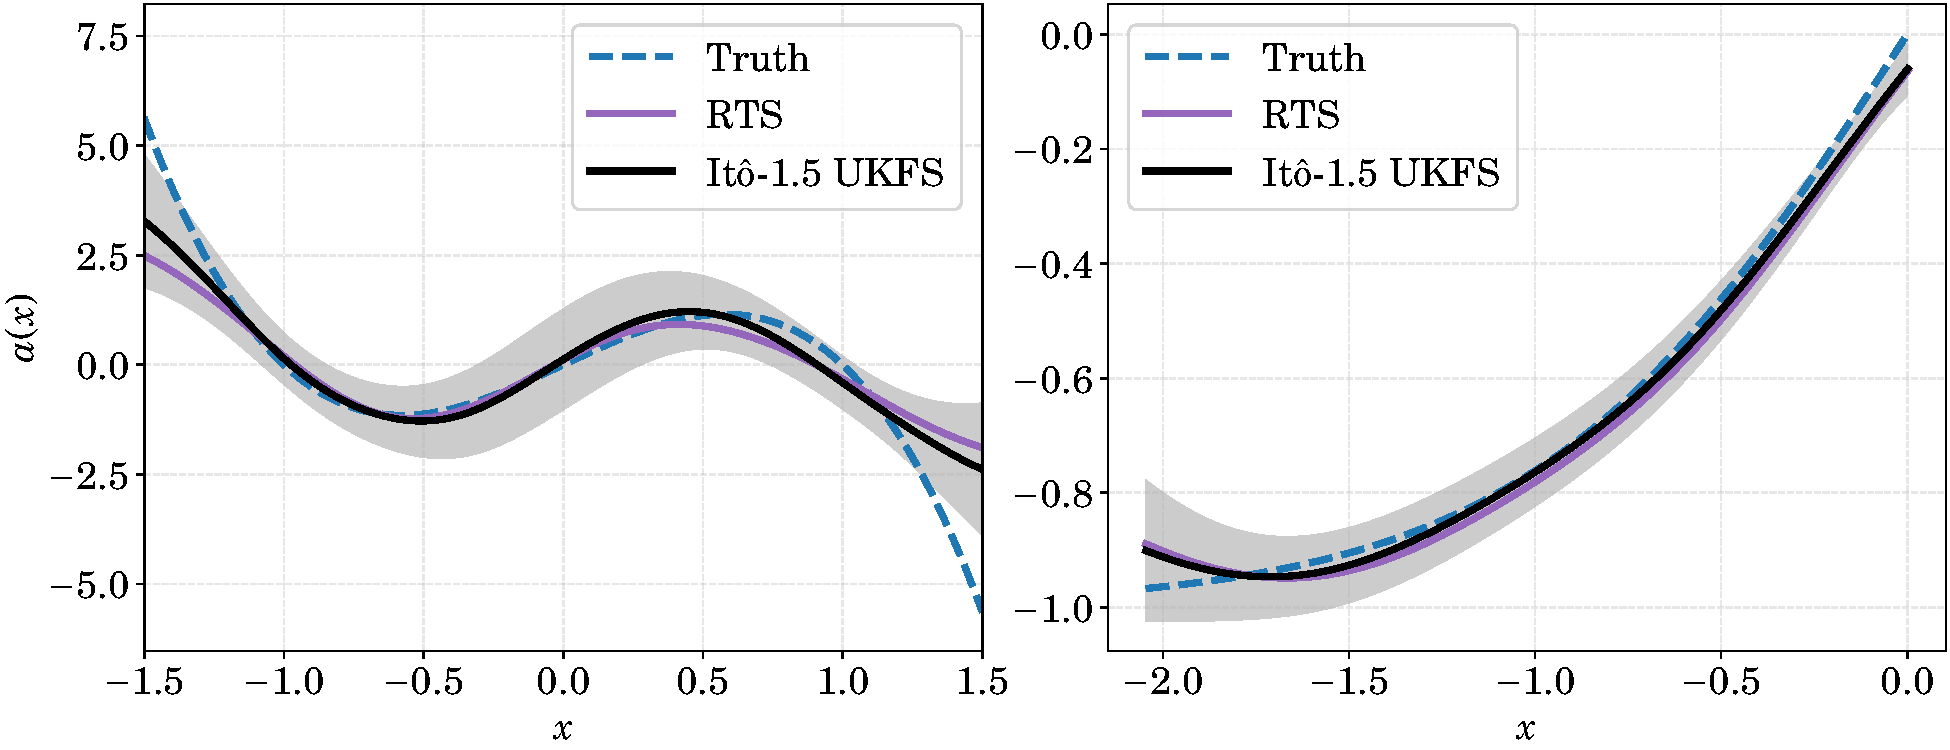
\includegraphics[width=.99\linewidth]{figs/drift-est}
	\caption{Estimation of drift functions $a(x)=3\,(x-x^3)$ (left) and $a(x)=\tanh(x)$ (right) by \citet{ZhaoZheng2020Drift}. UKFS stands for unscented Kalman filter and RTS smoother (UKFS). Shaded area stands for 0.95 confidence interval associated with the UKFS estimation.}
	\label{fig:drift-est}
\end{figure}

\citet{ZhaoZheng2020Drift} address the problems above by considering solving the GP regression problem in Equation~\eqref{equ:drift-est-reg-model} under the state-space framework. More precisely, they put an SS-GP prior over the unknown $a$ instead of a standard batch GP. The main benefit of doing so for this application is that the SS-GP regression solvers are computationally more efficient for large-scale measurements compared to the standard batch GP regression (see, Introduction and Section~\ref{sec:ssgp}). Moreover, in order to use high order It\^{o}--Taylor expansions, \citet{ZhaoZheng2020Drift} consider putting SS-GP priors over $a$ of the \matern family, so that the derivatives of $a$ naturally appear as the state components of $a$ (see, Section~\ref{sec:deep-matern}). In this way, computing the covariance matrices of the derivatives of $a$ is no longer needed.

\begin{remark}
	Note that the SS-GP approach requires to treat $X(t_1), X(t_2), \ldots ,\allowbreak X(t_T)$ as time variables and sort their data $x_{1:T}=\lbrace x_1,x_2,\ldots,x_T \rbrace$ in temporal order. 
\end{remark}

In Figure~\ref{fig:drift-est}, we show a representative result from~\citet{ZhaoZheng2020Drift}, where the SS-GP approach is employed to approximate the drift functions of two SDEs. In particular, the solutions are obtained by using the It\^{o}-1.5 discretisation, and an unscented Kalman filter and an RTS smoother. For more details regarding the experiments the reader is referred to~\citet{ZhaoZheng2020Drift}.

\section{Probabilistic spectro-temporal signal analysis}
\label{sec:spectro-temporal}
Let $z\colon \T \to \R$ be a periodic signal. In signal processing, it is often of interest to approximate the signal by Fourier expansions of the form
%
\begin{equation}
	z(t) \approx \alpha_0 + \sum^{N}_{n=1} \big[\alpha_n \cos(2 \, \pi \, \mathring{f}_n \, t) + \beta_n \sin(2 \, \pi \, \mathring{f}_n \, t)\big],
\end{equation}
%
where $\big\lbrace \mathring{f}_n\colon n=1,2,\ldots,N \big\rbrace$ stand for the frequency components, and $N$ is a given expansion order. When $z$ satisfies certain conditions~\citep{Katznelson2004}, the representation in the equation above converges as $N\to\infty$ (in various modes). 

Let use denote $y_k\coloneqq y(t_k)$ and suppose that we have a set of measurement data $y_{1:T}=\lbrace y_k\colon k=1,2,\ldots,T \rbrace$ of the signal at time instances $t_1, t_2, \ldots, t_T\in\T$. In order to quantify the truncation and measurement errors, we introduce Gaussian random variables $\xi_k \sim \mathrm{N}(0, \Xi_k)$ for $k=1,2,\ldots,T$ and let
%
\begin{equation}
	\begin{split}
		Y_k = \alpha_0 + \sum^{N}_{n=1} \big[\alpha_n \cos(2 \, \pi \, \mathring{f}_n \, t_k) + \beta_n \sin(2 \, \pi \, \mathring{f}_n \, t_k)\big] + \xi_k
		\label{equ:spectro-temporal-y}
	\end{split}
\end{equation}
%
represent the random measurements of $z$ at $t_k$. The goal now is to estimate the coefficients $\lbrace \alpha_0, \alpha_n, \beta_n \colon n=1,2,\ldots, N \rbrace$ from the data $y_{1:T}$. We call this problem the \emph{spectro-temporal estimation} problem.

One way to proceed is by using the MLE method~\citep{Bretthorst1988}, but~\citet{QiYuan2002, ZhaoZheng2018KF, ZhaoZheng2020KFECG} show that we can also consider this spectro-temporal estimation problem as a GP regression problem. More precisely, the modelling assumption is that
%
\begin{equation}
	\begin{split}
		\alpha_0(t) &\sim \mathrm{GP}\big(0, C^0_\alpha(t, t')\big),\\
		\alpha_n(t) &\sim \mathrm{GP}\big(0, C^n_\alpha(t, t')\big),\\
		\beta_n(t) &\sim \mathrm{GP}\big(0, C^n_\beta(t, t')\big),
		\label{equ:spectro-temporal-gp-priors}
	\end{split}
\end{equation}
%
for $n=1,2,\ldots, N$, and that the measurements follow
%
\begin{equation}
	Y_k = \alpha_0(t_k) + \sum^{N}_{n=1} \big[\alpha_n(t_k) \, \cos(2 \, \pi \, \mathring{f}_n \, t_k) + \beta_n(t_k) \, \sin(2 \, \pi \, \mathring{f}_n \, t_k)\big] + \xi_k,\nonumber
\end{equation}
%
for $k=1,2,\ldots,T$. This results in a standard GP regression problem therefore, the posterior distribution of coefficients $\lbrace \alpha_0, \alpha_n, \beta_n \colon n=1,2,\ldots, N \rbrace$ have a close-form solution. However, solving this GP regression problem is, in practice, infeasible when the expansion order $N$ and the number of measurements $T$ are large. This is due to the fact that one needs to compute $2\,N+1$ covariance matrices of dimension $T\times T$ and compute their inverse.

\citet{ZhaoZheng2018KF} propose to solve this spectro-temporal GP regression problem under the state-space framework, that is, by replacing the GP priors in Equation~\eqref{equ:spectro-temporal-gp-priors} with their SDE representations. Since SS-GPs have already been extensively discussed in previous sections, we omit the resulting state-space spectro-temporal estimation formulations. However, the details can be found in Section~\ref{sec:ssgp} and in~\citet{ZhaoZheng2018KF}.

The computational cost of the state-space spectro-temporal estimation method is substantially cheaper than that of standard batch GP methods. Indeed, Kalman filters and smoothers only need to compute one $E$-dimensional covariance matrix at each time step (see, Algorithm~\ref{alg:kfs}) instead of those required by batch GP methods. The dimension $E$ is equal to the sum of all the state dimensions of the SS-GPs $\lbrace \alpha_0, \alpha_n, \beta_n \colon n=1,2,\ldots, N \rbrace$. 

\citet{ZhaoZheng2020KFECG} further extend the state-space spectro-temporal estimation method by putting quasi-periodic SDE priors~\citep{Solin2014} over the Fourier coefficients instead of the Ornstein--Uhlenbeck SDE priors used in~\citet{ZhaoZheng2018KF}. This consideration generates a time-invariant version of the measurement model in Equation~\eqref{equ:spectro-temporal-y}, thus, one can apply steady-state Kalman filters and smoothers (SS-KFSs) in order to achieve lower computational costs. The computational cost is further reduced because SS-KFSs do not need to compute the $E$-dimensional covariances of the state in their filtering and smoothing loops. Instead, the state covariances in SS-KFSs are replaced by a pre-computed steady covariance matrix obtained as the solution of its discrete algebraic Riccati equation (DARE). Moreover, solving the DARE is independent of data/measurements, which is especially useful when the model is known or fixed. However, SS-KFSs may not always be computationally efficient when $N \gg T$, since solving an $E$-dimensional DARE can be demanding when $E$ is large.

\citet{ZhaoZheng2018KF, ZhaoZheng2020KFECG} show that the state-space spectro-temporal estimation method can be a useful feature extraction mechanism for detecting atrial fibrillation from electrocardiogram signals. More specifically, the spectro-temporal method estimates the spectrogram images of atrial fibrillation signals. These images are then fed to a deep convolutional neural network classifier which is tasked with recognising atrial fibrillation manifestations.

Since the measurement noises $\lbrace \xi_k\colon k=1,2,\ldots,T \rbrace$ in Equation~\eqref{equ:spectro-temporal-y} encode the truncation and measurement errors, it is also of interest to estimate them. This is done in~\citet{GaoRui2019ALKS}, where the variances $\Xi_k$ of $\xi_k$ for $k=1,2,\ldots, T$ are estimated under the alternating direction method of multipliers.

\begin{figure}[t!]
	\centering
	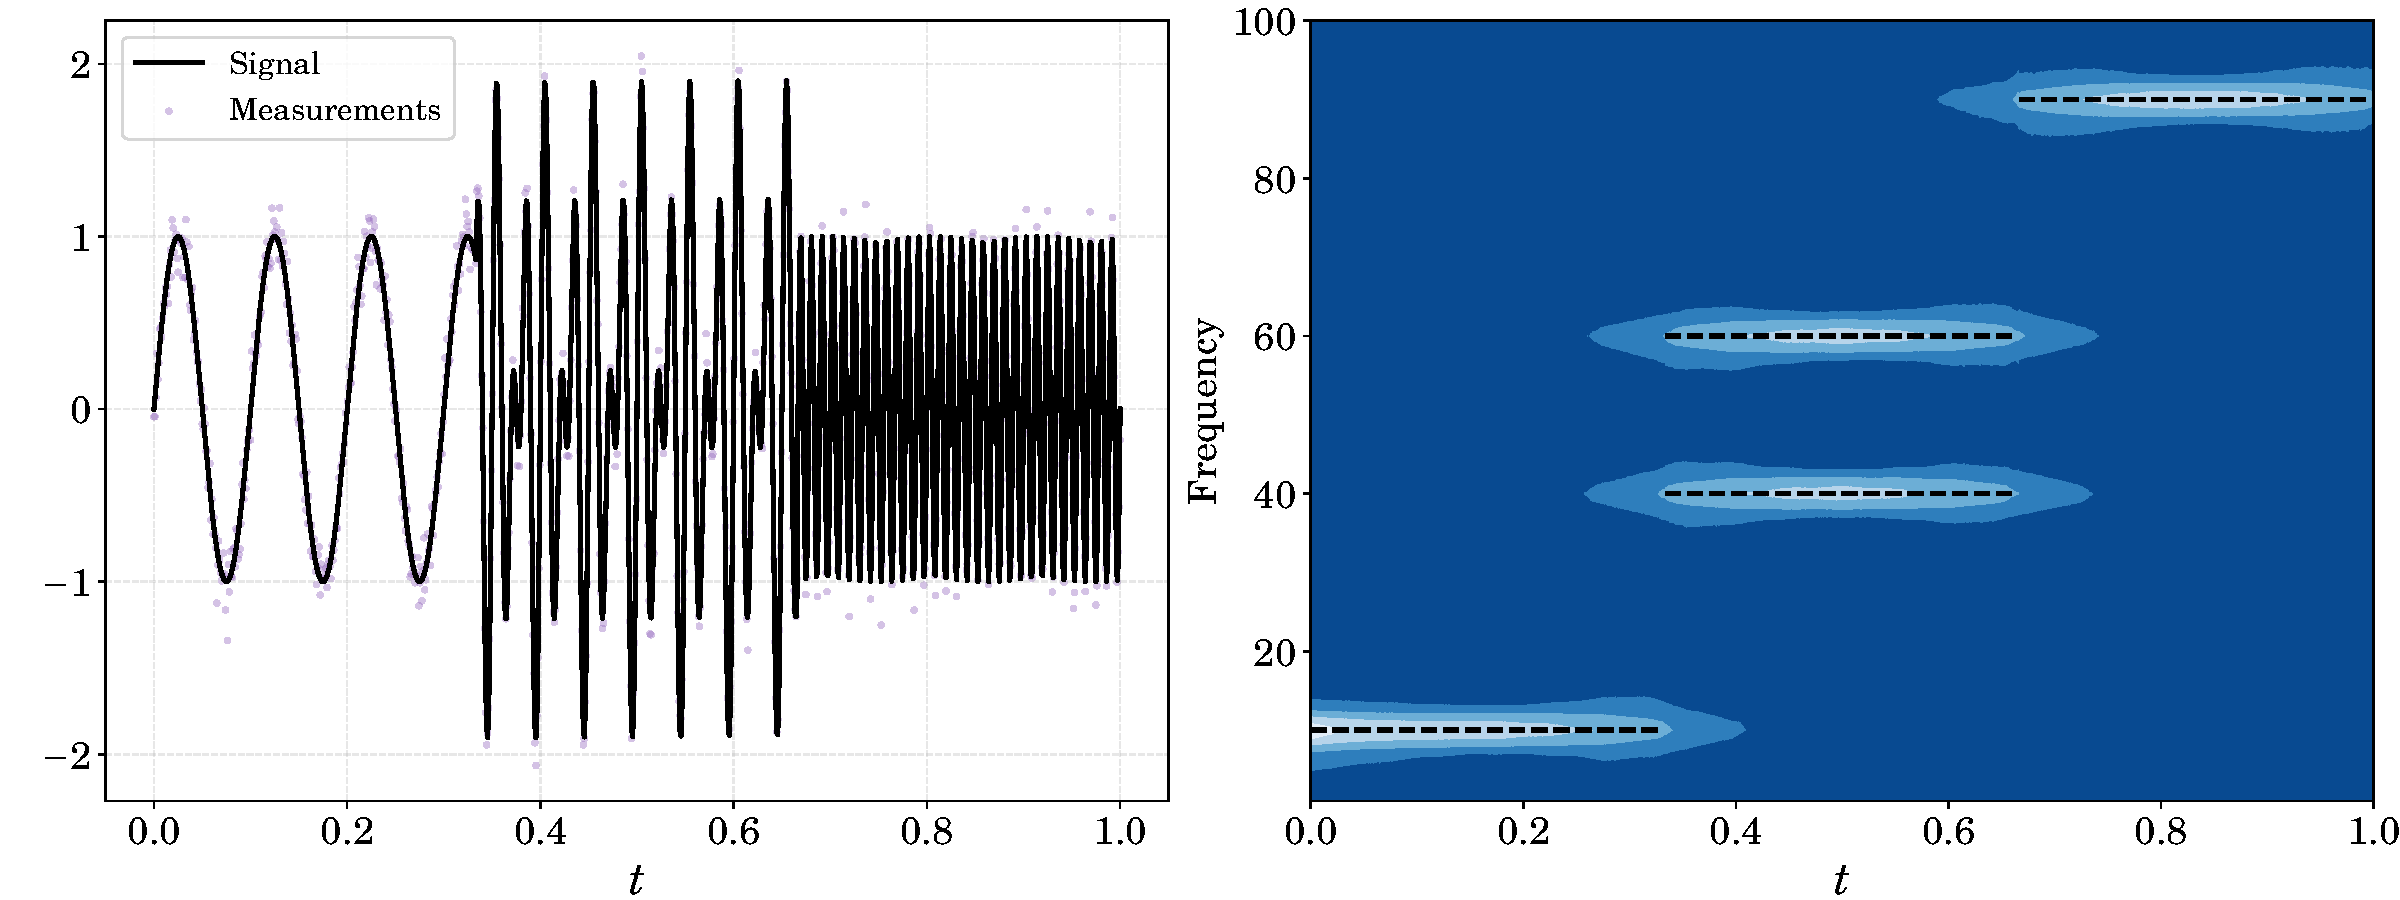
\includegraphics[width=.99\linewidth]{figs/spectro-temporal-demo1}
	\caption{Spectrogram (right, contour plot) of a sinusoidal signal (left) generated by Kalman filtering and RTS smoothing using the method in Section~\ref{sec:spectro-temporal}. Dashed black lines (right) stand for the ground truth frequencies.}
	\label{fig:spectro-temporal-demo}
\end{figure}

Figure~\ref{fig:spectro-temporal-demo} illustrates an example of using the state-space spectro-temporal estimation method to estimate the spectrogram of a sinusoidal signal with multiple frequency bands. 

\section{Signal modelling with SS-DGPs}
\label{sec:apps-ssdgp}
In this section, we apply SS-DGPs for modelling gravitational waves and human motion (i.e., acceleration). We consider these as SS-DGP regression problems, where the measurement models are assumed to be linear with respect to the SS-DGPs with additive Gaussian noises. As for their priors, we chose the Mat\'{e}rn $\nu=3 \, / \, 2$ SS-DGP in Example~\ref{example:ssdgp-m32}, except that the parent GPs $U^2_1$ and $U^3_1$ use the Mat\'{e}rn $\nu=1 \, / \, 2$ representation.

\subsection*{Modelling gravitational waves}
Gravitational waves are curvatures of spacetime caused by the movement of objects with mass~\citep{Maggiore2008}. Since the time Albert Einstein predicted the existence of gravitational waves theoretically from a linearised field equation in 1916~\citep{EinsteinGW1937, Hill2017}, much effort has been done to observe their presence~\citep{Blair1991}. In 2015, the laser interferometer gravitational-wave observatory (LIGO) team first observed a gravitational wave from the merging of a black hole binary~\citep[event GW150914,][]{LIGO2016}. This wave/signal is challenging for standard GPs to fit because the frequency of the signal changes over time. It is then of our interest to see if SS-DGPs can fit this gravitational wave signal.

\begin{figure}[t!]
	\centering
	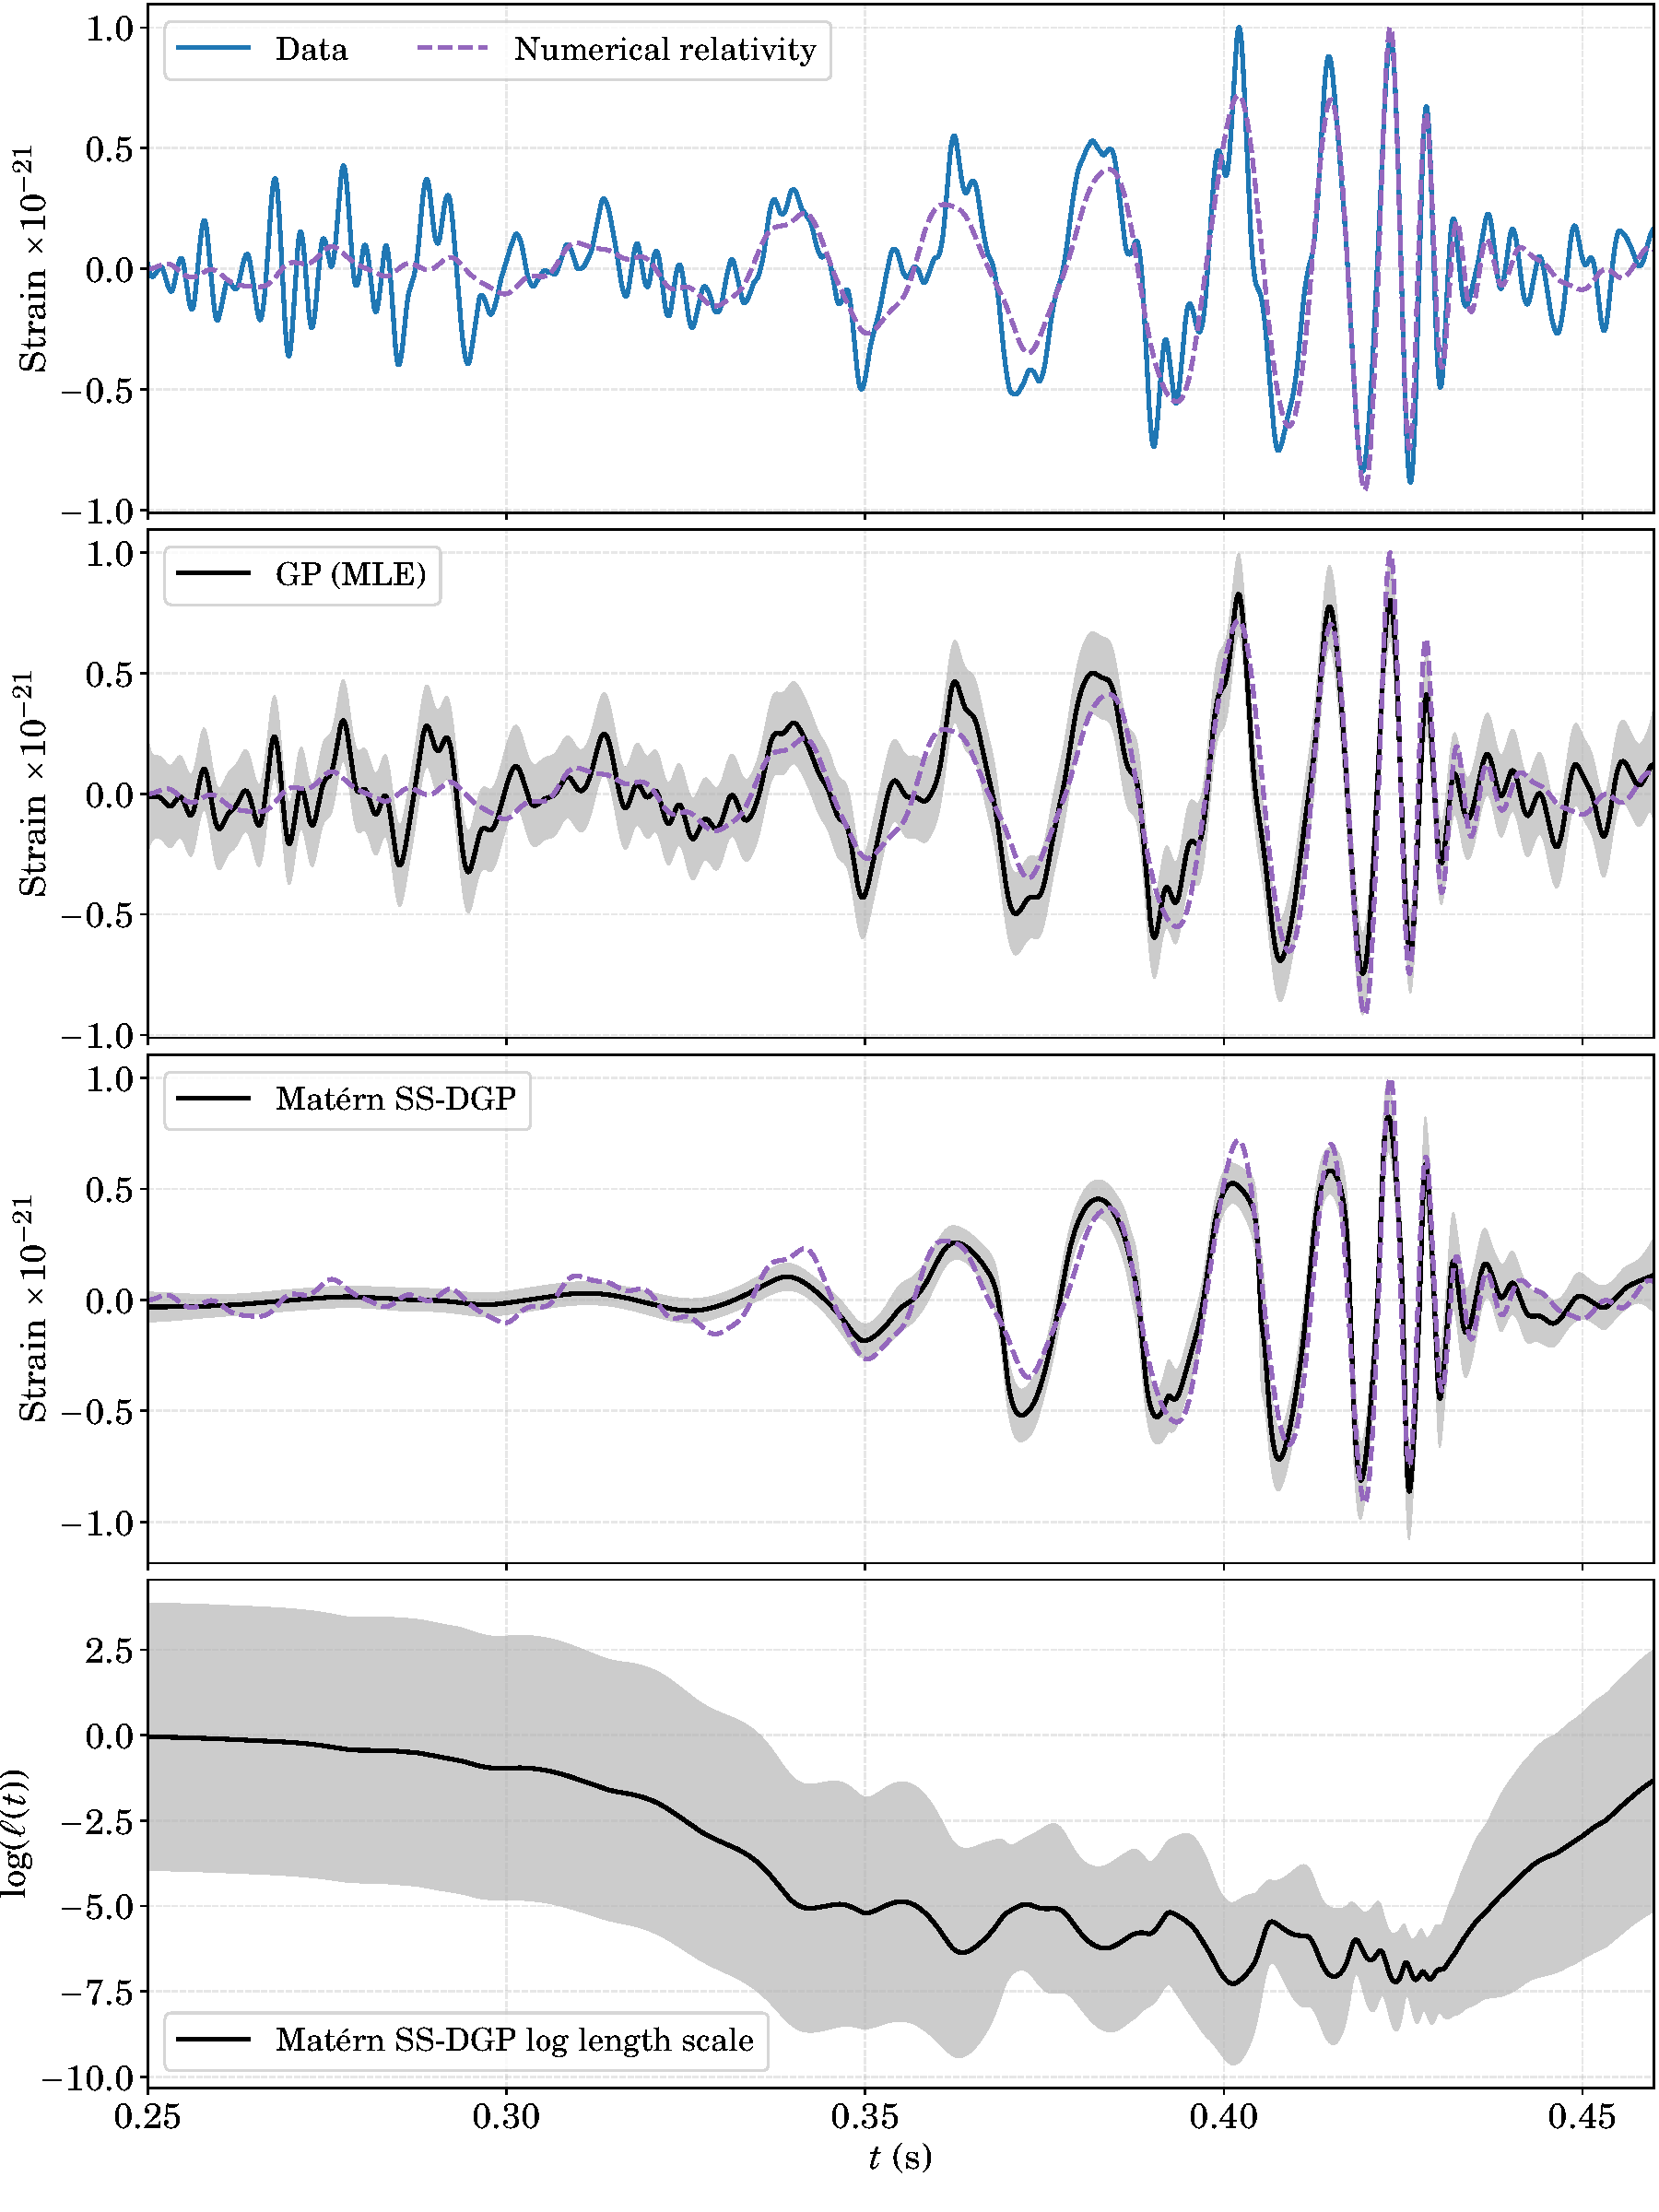
\includegraphics[width=.99\linewidth]{figs/gravit-wave-ssdgp}
	\caption{Mat\'{e}rn $\nu=3\, \, /\, 2$ SS-DGP regression (solved by cubature Kalman filter and smoother) for the gravitational wave in event GW150914 (Hanford, Washington). The shaded area stands for 0.95 confidence interval. Details about the data can be found in~\citet{Zhao2020SSDGP}.}
	\label{fig:gravit-wave-ssdgp}
\end{figure}

Figure~\ref{fig:gravit-wave-ssdgp} plots the SS-DGP fit for the gravitational wave observed in the event GW150914. In the same figure, we also show the fit from a \matern $\nu=3\,/\,2$ GP as well as a waveform (which is regarded as the ground truth) computed from the numerical relativity (purple dashed lines) for comparison. Details about the experiment and data are found in~\citet{Zhao2020SSDGP}.

Figure~\ref{fig:gravit-wave-ssdgp} shows that the GP fails to give a reasonable fit to the gravitational wave because the GP over-adapts the high-frequency section of the signal around $0.4$~s. On the contrary, the SS-DGP does not have such a problem, and the fit is closer to the numerical relativity waveform compared that of the GP. Moreover, the estimated length scale (in log transformation) can interpret the data in the sense that the length scale value decreases as the signal frequency increases. 

\subsection*{Modelling human motion}
We apply the regularised SS-DGP (R-SS-DGP) presented in Section~\ref{sec:l1-r-dgp} to fit an accelerometer recording of human motion. The reason for using R-SS-DGP here is that the recording (see, the first row of Figure~\ref{fig:imu-r-ssdgp}) is found to have some sharp changes and artefacts. Hence, we aim at testing if we can use sparse length scale and magnitude to describe such data. The collection of accelerometer recordings and the experiment settings are detailed in~\citet{Hostettler2018} and~\citet{Zhao2021RSSGP}, respectively.

\begin{figure}[t!]
	\centering
	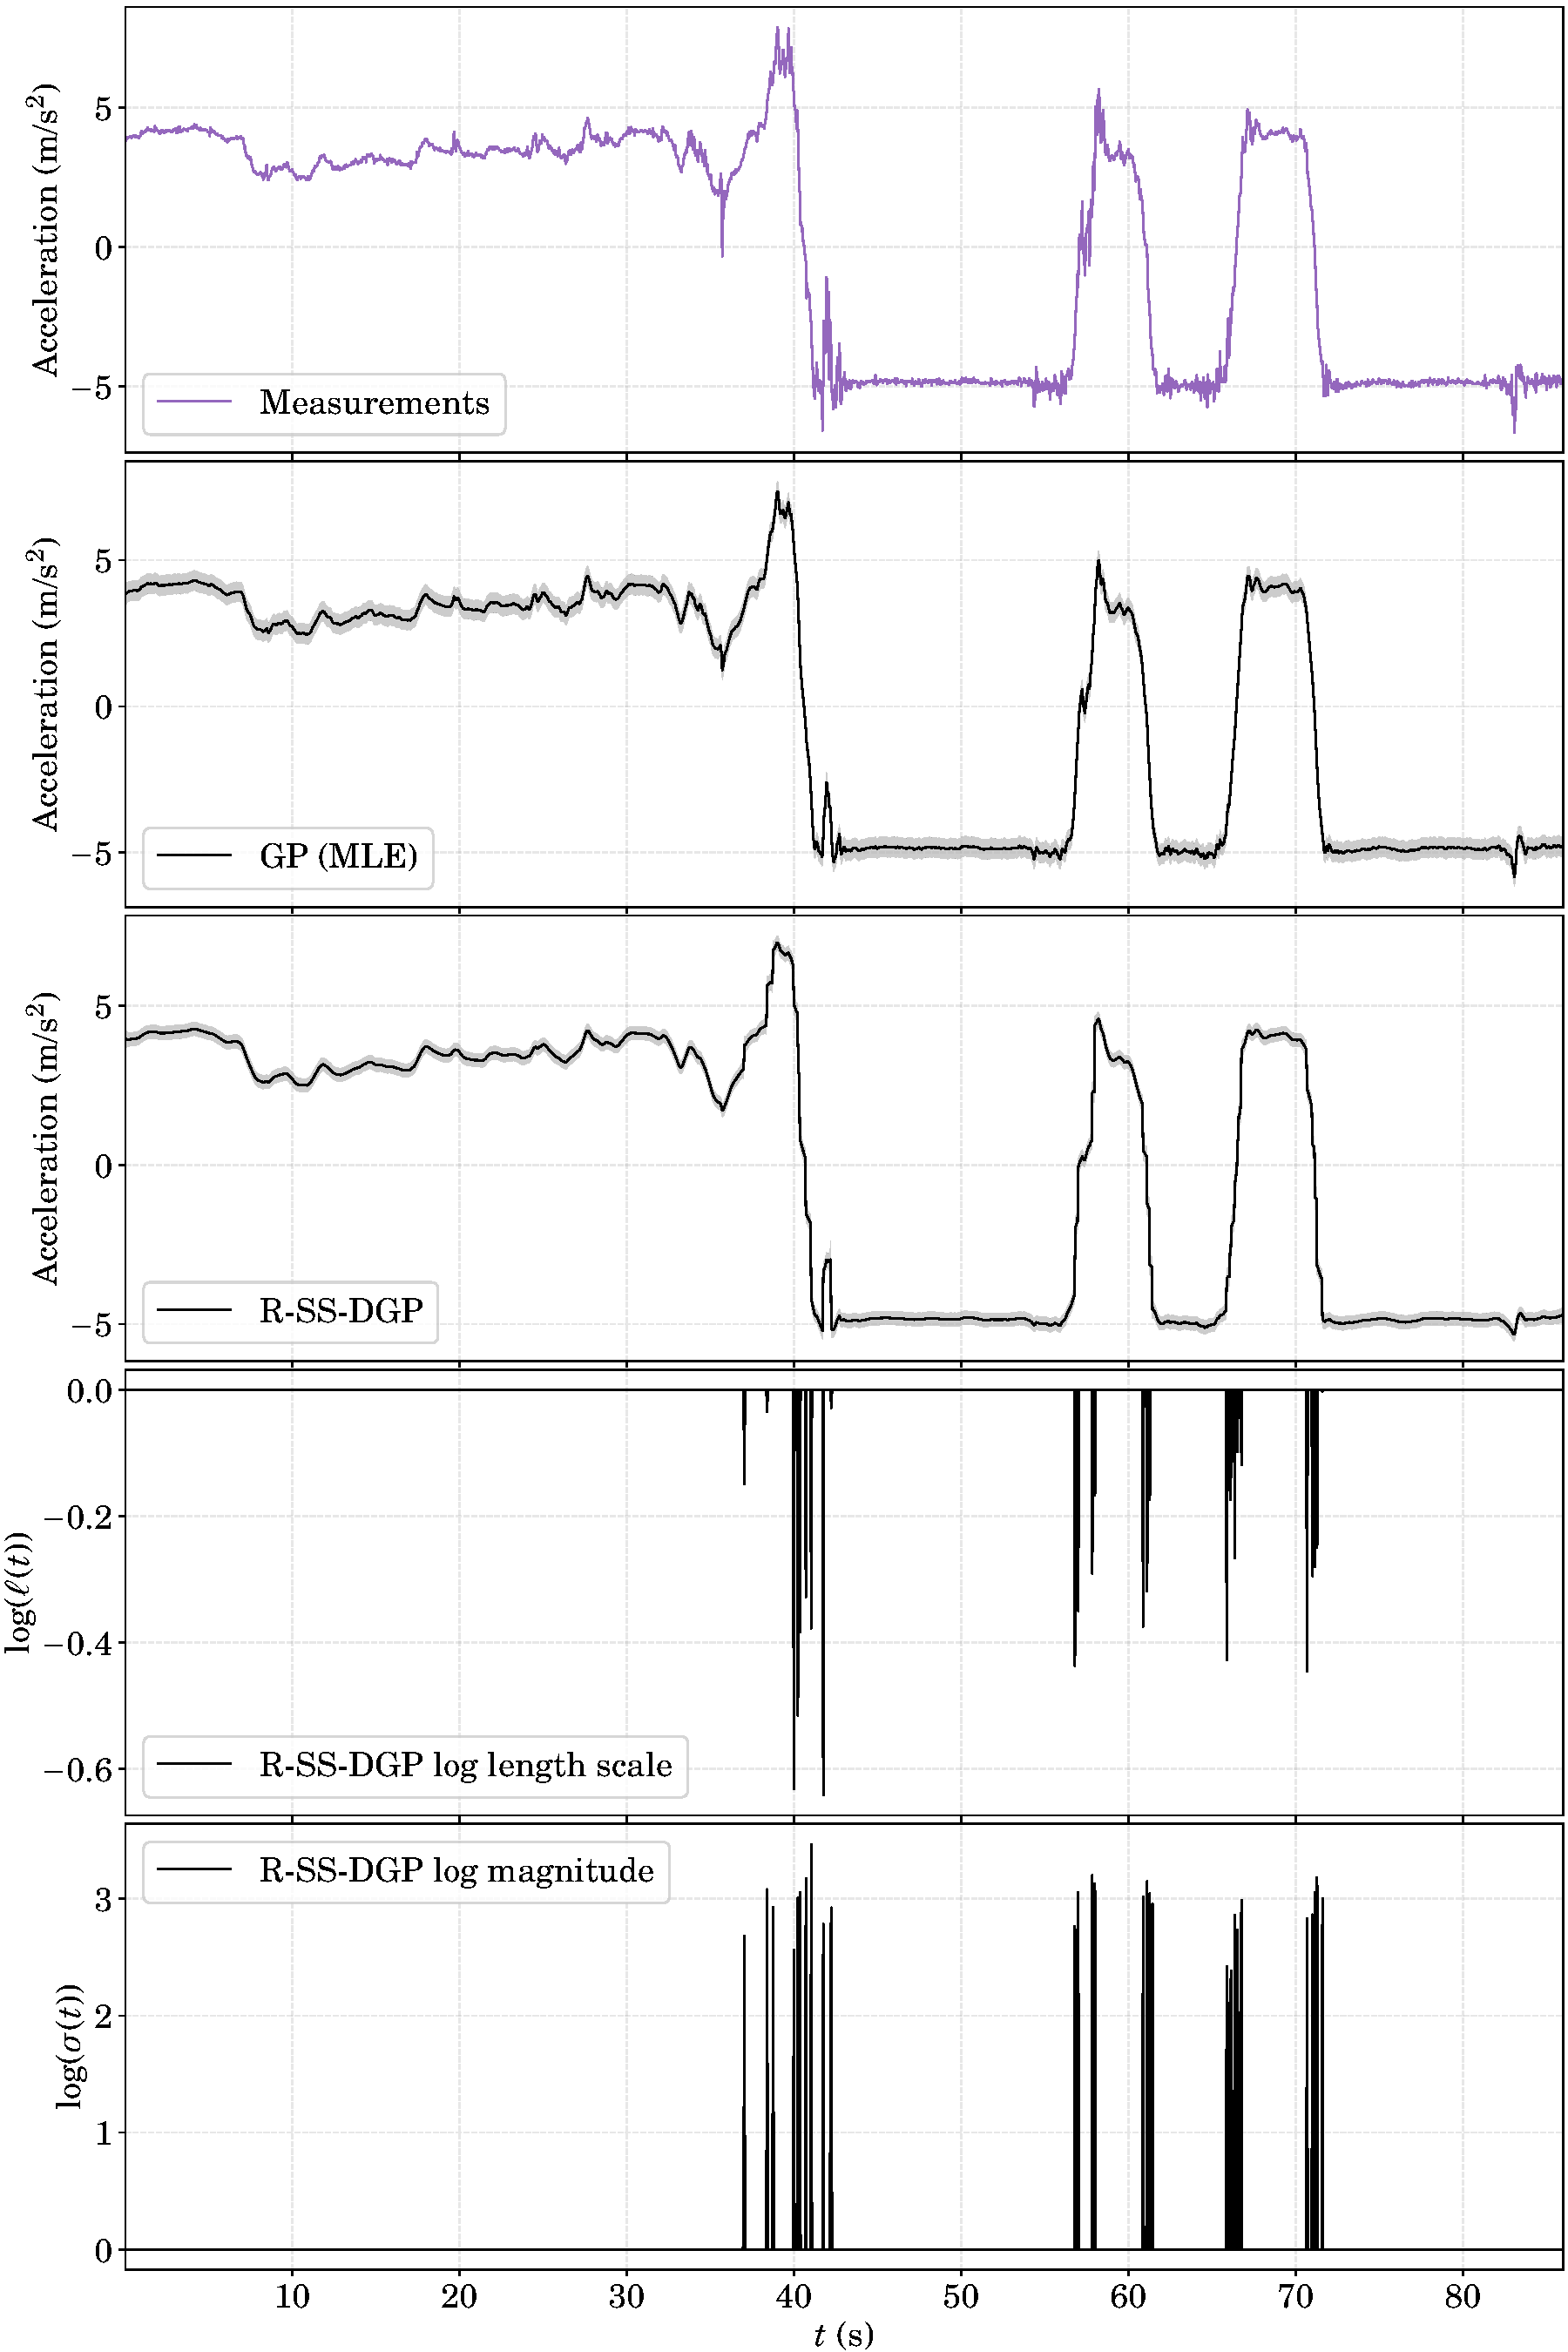
\includegraphics[width=.99\linewidth]{figs/imu-r-ssdgp}
	\caption{Human motion modelling with an R-SS-DGP. The GP here uses a \matern $\nu=3\,/\,2$ covariance function. Shaded area stands for 0.95 confidence interval.}
	\label{fig:imu-r-ssdgp}
\end{figure}

A demonstrative result is shown in Figure~\ref{fig:imu-r-ssdgp}. We see that the fit of R-SS-DGP is smoother than that of GP. Moreover, the posterior variance of R-SS-DGP is also found to be reasonably smaller than GP. It is also evidenced from the figure that the GP does not handle the artefacts well, for example, around times $t=55$~s and $62$~s. Finally, we find that the learnt length scale and magnitude (in log transformation) are sparse, and that they can respond sharply to the abrupt signal changes and artefacts.

\section{Maritime situational awareness}
\label{sec:maritime}
Another area of applications of (deep) GPs is  autonomous maritime navigation. In~\citet{Sarang2020}, we present a literature review on the sensor technology and machine learning methods for autonomous vessel navigation. In particular, we show that GP-based methods are able to analyse ship trajectories~\citep{Rong2019}, detect navigation abnormality~\citep{Kowalska2012, Smith2014}, and detect/classify vessels~\citep{XiaoZ2017}.

\begin{figure}[t!]
	\centering
	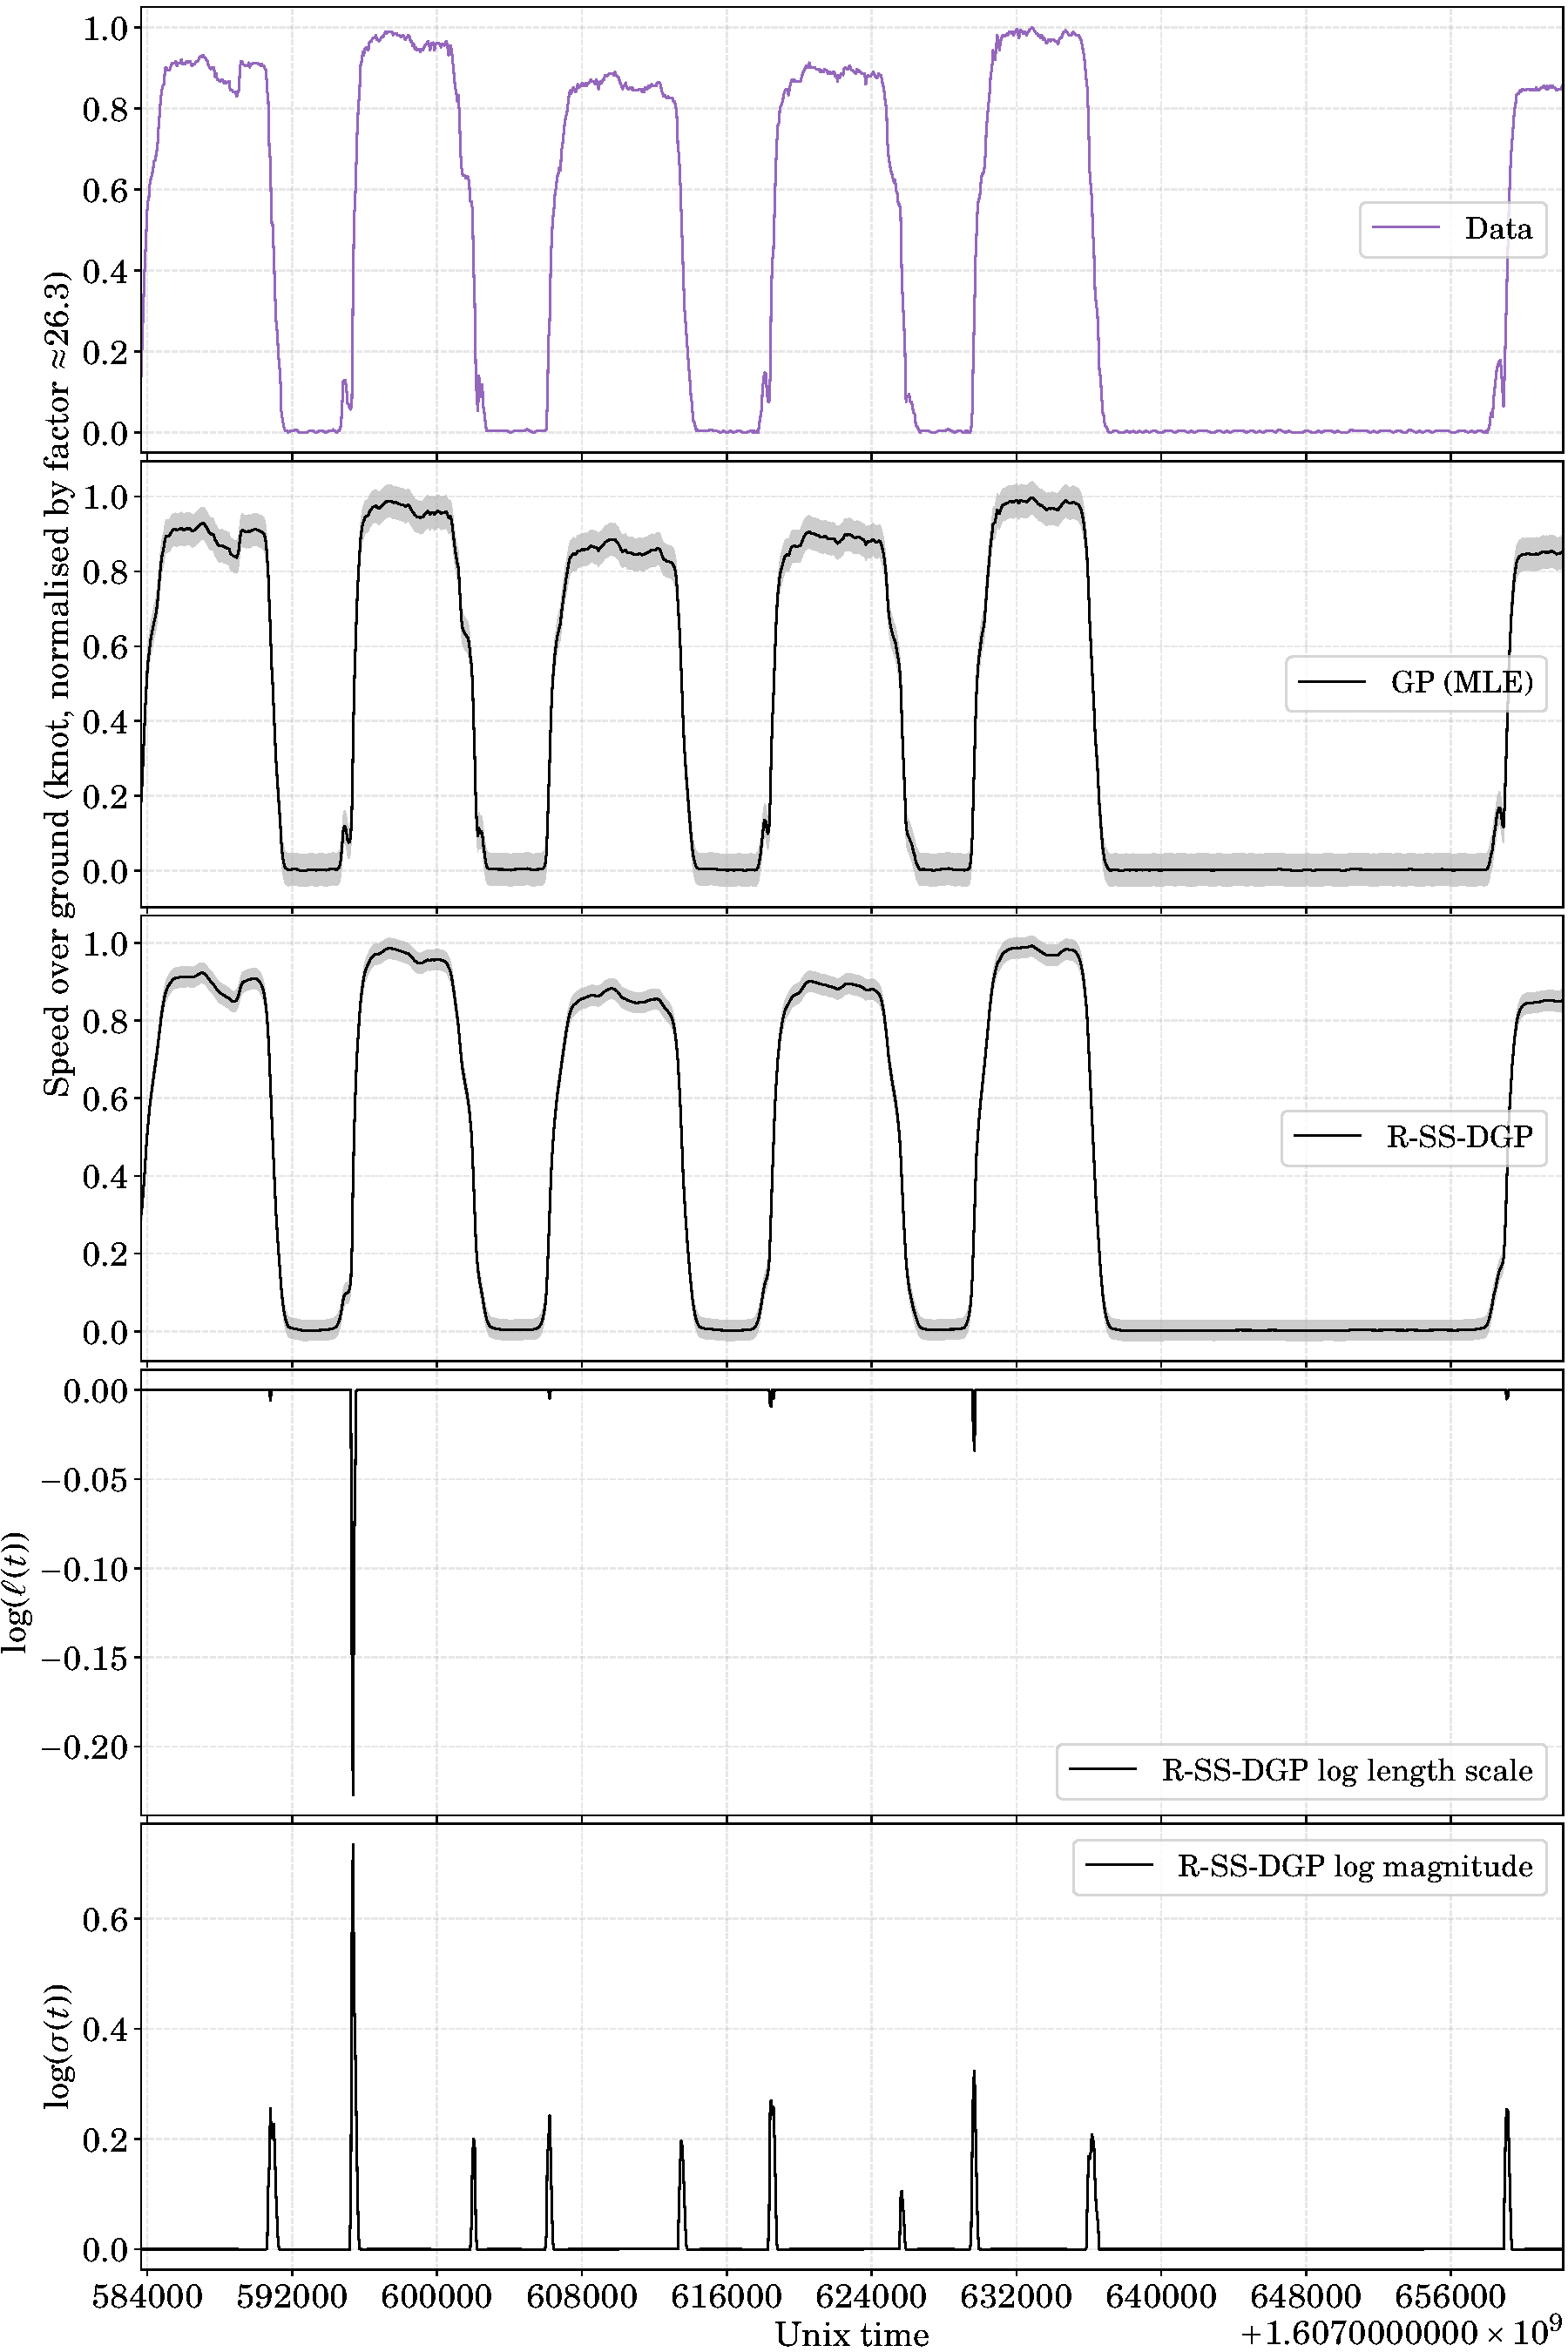
\includegraphics[width=.99\linewidth]{figs/ais-r-ssdgp}
	\caption{Modelling AIS recording (speed over ground) of MS Finlandia with an R-SS-DGP. The GP here uses a \matern $\nu=3\,/\,2$ covariance function. Shaded area stands for 0.95 confidence interval.}
	\label{fig:ais-ssdgp}
\end{figure}

In Figure~\ref{fig:ais-ssdgp}, we present an example for fitting an automatic identification system (AIS) recording by using an R-SS-DGP. The recording is taken from MS Finlandia (Helsinki--Tallinn) by Fleetrange Oy on December 10, 2020. We see from the figure that the fit of R-SS-DGP is smoother than that of GP. Moreover, the learnt length scale and magnitude parameters are flat and jump at the acceleration/deceleration points.
